\begin{itemize}
	\item ограничить сечение рассеяния можно зная: конечное распределение ($aT_{\odot}^2$), огрпничение на тема аннигиляции в нейтрино $A$. 
\end{itemize}
\begin{figure}[!h]
	\centering
	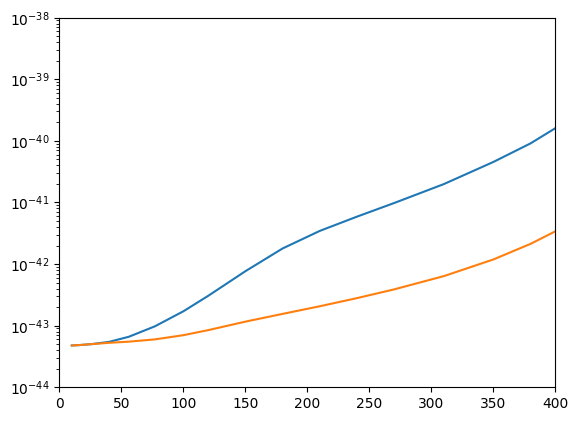
\includegraphics[width=0.65\textwidth]{images/Constrains.png}
	\caption{Пример ограничений из IC. Канал $\chi+\chi \to W^{+} + W^{-}$}
\end{figure}